\chapter{Perfiles de estudiantes según su rendimiento}
\addcontentsline{toc}{chapter}{Perfiles de estudiantes según su rendimiento}

Debido a la dificultad de predecir de manera exacta la calificación obtenida por los alumnos a partir de las medidas de rendimiento descritas anteriormente, se agruparán las notas en clusters significativos y trataremos de predecir en qué cluster se encuentra la nota de un determinado grupo de alumnos.

\section{Por clusters fijos de notas}

En primer lugar, escogeremos como separación los cuartiles de las calificaciones. Así pues, podemos ver la distribución de los cuartiles en la Figura \ref{fig:boxplotquartilegrade}, donde los límites inferiores de cada una de las cajas son $6.99$, $8.23$, $8.95$ y $9.60$ respectivamente. También puede verse en la Figura \ref{fig:countquartilegrade} el número de grupos que hay en cada cuartil.


\begin{figure}[H]
\centering
\subfloat[Boxplot de las calificaciones por cuartil.]{\label{fig:boxplotquartilegrade}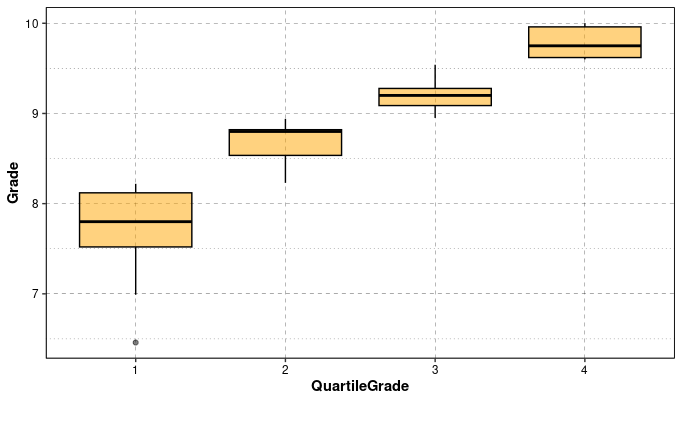
\includegraphics[width=0.47\textwidth]{clustering/boxplotgrade.png}}\qquad
\subfloat[Número de grupos por cuartil.]{\label{fig:countquartilegrade}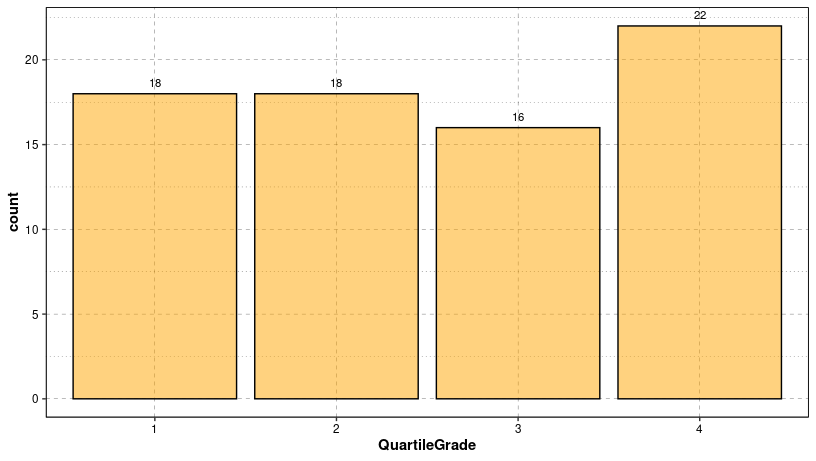
\includegraphics[width=0.47\textwidth]{clustering/countquartilegrade.png}}%
\caption{Resultados obtenidos tras aplicar el algoritmo agrupar las caficaciones por cuartiles.}
\label{fig:quartilegradeclustering}
\end{figure}

Sin embargo, en la Figura \ref{fig:boxplotquartilegrade} y en la Figura \ref{fig:frequenciesgrade}, donde se representan cómo de frecuentes son cada una de las calificaciones obtenidas, notamos la presencia de un outlier.

\begin{figure}[H]
    \centering
    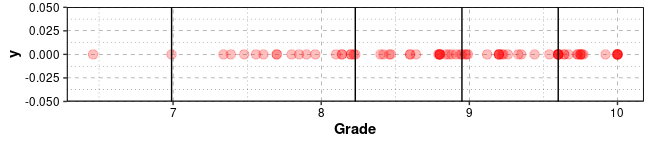
\includegraphics[width=0.6\textwidth]{clustering/frequencygrade.png}
    \caption{Calificaciones obtenidas por los distintos grupos. El límite de los cuartiles se ha indicado con líneas verticales negras.}
    \label{fig:frequenciesgrade}
\end{figure}

En la Figura \ref{fig:densitybyfactorquartilegrade} vemos las funciones de densidad por cuartil. Prestaremos especial atención a los grupos del cluster \texttt{Q1} (el de las peores calificaciones al que le añadimos el outlier) puesto que son los que peor rendimiento han mostrado.

\begin{figure}[H]
    \centering
    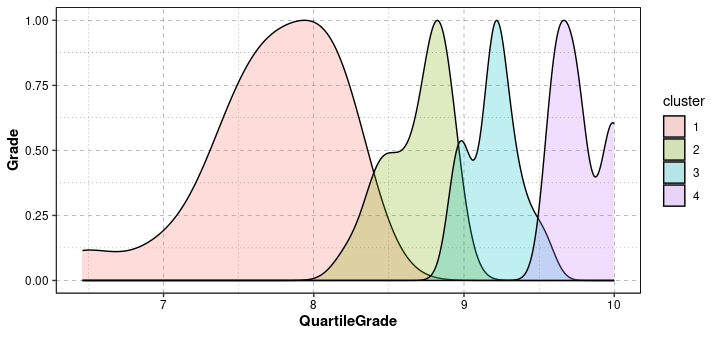
\includegraphics[width=0.6\textwidth]{clustering/densitybyfactorquartilegrade.png}
    \caption{Funciones de densidad de las calificaciones obtenidas por cluster.}
    \label{fig:densitybyfactorquartilegrade}
\end{figure}

\section{Por clusters dinámicos de notas}

Se agruparán los datos usando el algoritmo de las K-medias sobre la variable \emph{Grade}. Para decidir el número de clusters en el que agruparemos los datos, se usarán métodos gráficos. Como podemos ver en las Figuras \ref{fig:indiceshubert} y \ref{fig:indicesdindex}, el número óptimo de particiones podría ser $3$ o $5$. Para decidir entre un número de clusters u otro se realizarán los dos agrupamientos y nos quedaremos con el de menor error.

\begin{figure}[H]
    \centering
    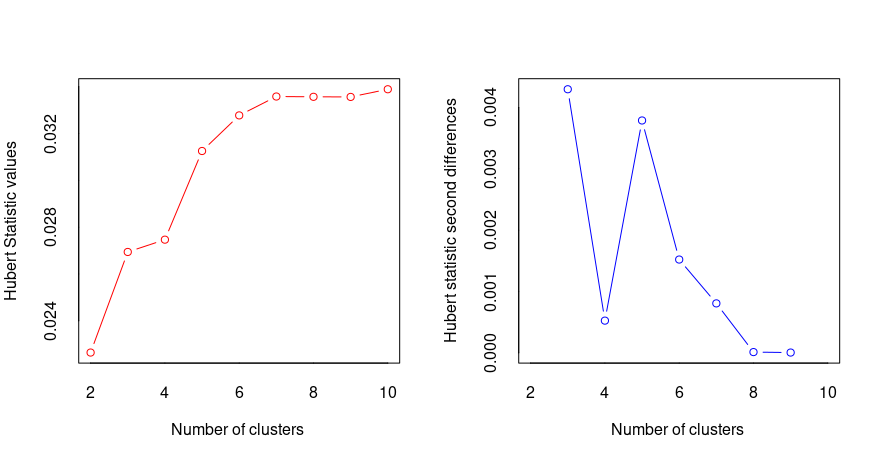
\includegraphics[width=\textwidth]{clustering/Hubert.png}
    \caption{Valores estadísticos de Hubert.}
    \label{fig:indiceshubert}
\end{figure}

\begin{figure}[H]
    \centering
    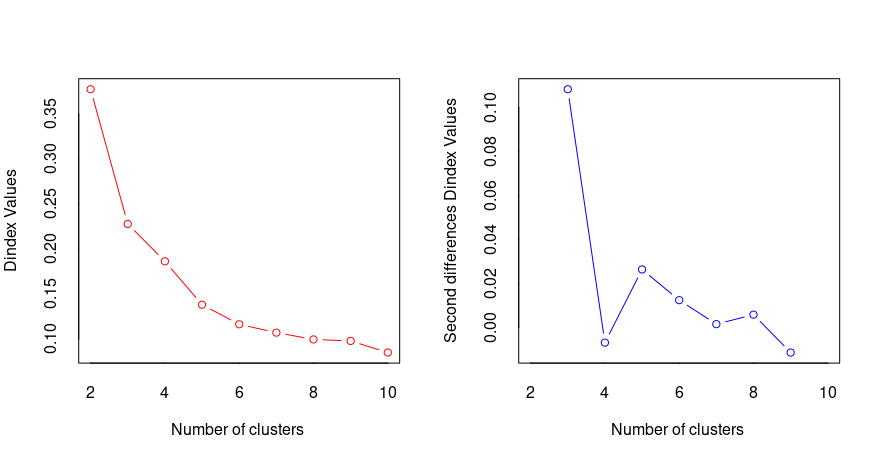
\includegraphics[width=\textwidth]{clustering/Dindex.png}
    \caption{Valores de Dindex.}
    \label{fig:indicesdindex}
\end{figure}

Aplicando el algoritmo de las K-medias para $K = 2$ (Figura \ref{fig:KMeans2}) y para $K = 3$ (Figura \ref{fig:KMeans3}), vemos que hay una gran diferencia la precisión de uno y otro (para $K = 2$ se tiene $\texttt{accuracy} = 0.6978412$ mientras que para $K = 3$ se tendrá $\texttt{accuracy} = 0.8585982$). Como podemos ver en la Figura \ref{fig:KMeans2}, seguimos teniendo un outlier.

\begin{figure}[H]
    \centering
    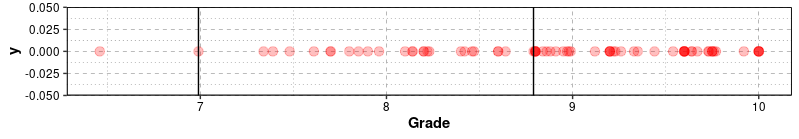
\includegraphics[width=0.6\textwidth]{clustering/KMeans2.png}
    \caption{Particiones obtenidas con $K = 2$.}
    \label{fig:KMeans2}
\end{figure}

\begin{figure}[H]
    \centering
    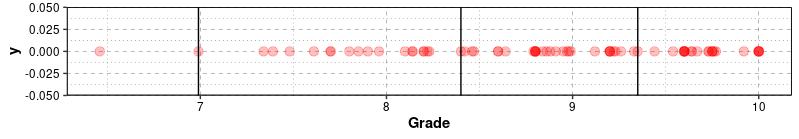
\includegraphics[width=0.6\textwidth]{clustering/KMeans3.png}
    \caption{Particiones obtenidas con $K = 3$.}
    \label{fig:KMeans3}
\end{figure}

La distribución de la variable \emph{Grade} dentro de cada partición puede verse en las Figuras \ref{fig:KMeans2boxplot} y \ref{fig:KMeans3boxplot} mientras que el número de grupo que hay en las particiones puede verse en las Figuras \ref{fig:KMeans2count} y \ref{fig:KMeans3count}.

\begin{figure}[H]
\centering
\subfloat[Boxplot de cada una de las particiones.]{\label{fig:KMeans2boxplot}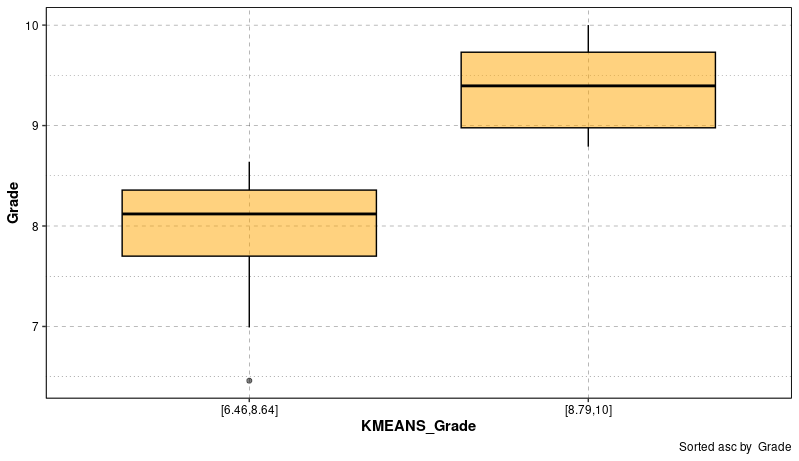
\includegraphics[width=0.47\textwidth]{clustering/KMeans2boxplot.png}}\qquad
\subfloat[Número de grupos por partición.]{\label{fig:KMeans2count}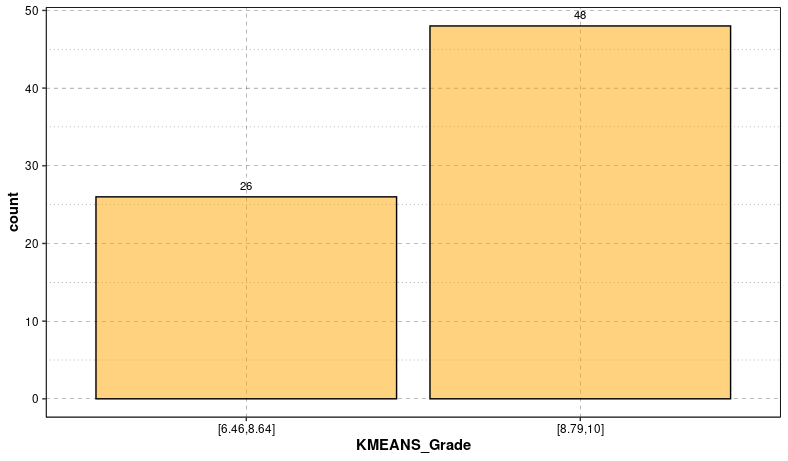
\includegraphics[width=0.47\textwidth]{clustering/KMeans2count.png}}%
\caption{Resultados obtenidos tras aplicar el algoritmo de las $K$-Medias con $K = 2$.}
\label{fig:KMeans2details}
\end{figure}

\begin{figure}[H]
\centering
\subfloat[Boxplot de cada una de las particiones.]{\label{fig:KMeans3boxplot}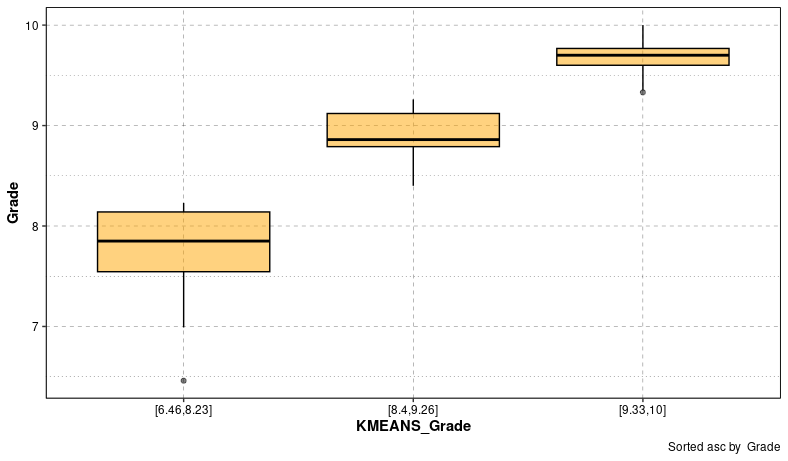
\includegraphics[width=0.47\textwidth]{clustering/KMeans3boxplot.png}}\qquad
\subfloat[Número de grupos por partición.]{\label{fig:KMeans3count}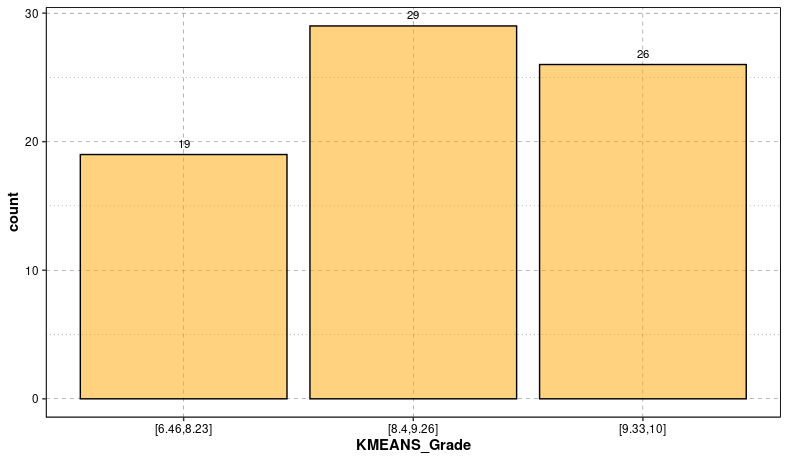
\includegraphics[width=0.47\textwidth]{clustering/KMeans3count.png}}%
\caption{Resultados obtenidos tras aplicar el algoritmo de las $K$-Medias con $K = 3$.}
\label{fig:KMeans3details}
\end{figure}

Por último, para cinco particiones (Figura \ref{fig:KMeans5}) se tendrá $\texttt{accuracy} = 0.9474439$. Es decir, tenemos más precisión con cinco particiones y ya no tenemos outliers. Nos centramos en estudiar los grupos de los dos primeros clusters (aquellos grupos con una nota inferior a $7.34$).

\begin{figure}[H]
    \centering
    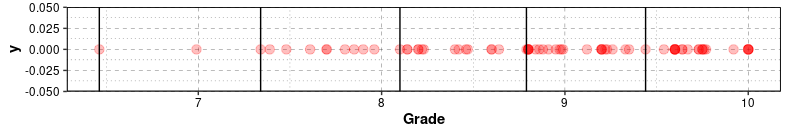
\includegraphics[width=0.6\textwidth]{clustering/KMeans5.png}
    \caption{Particiones obtenidas con $K = 5$.}
    \label{fig:KMeans5}
\end{figure}

\begin{figure}[H]
\centering
\subfloat[Boxplot de cada una de las particiones.]{\label{fig:KMeans5boxplot}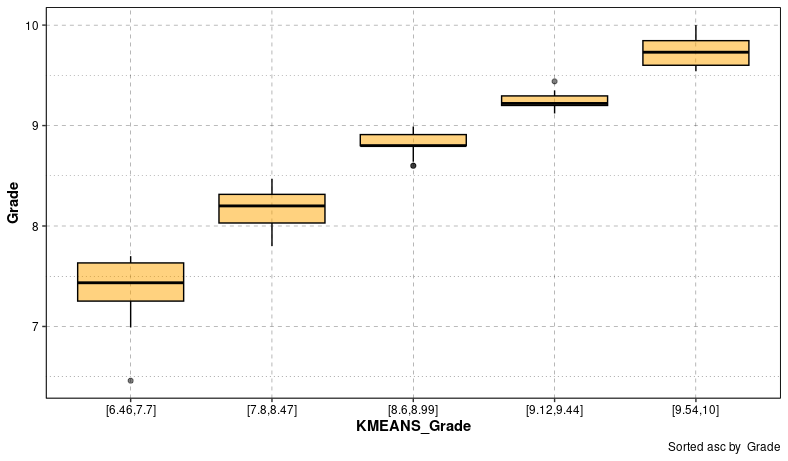
\includegraphics[width=0.47\textwidth]{clustering/KMeans5boxplot.png}}\qquad
\subfloat[Número de grupos por partición.]{\label{fig:KMeans5count}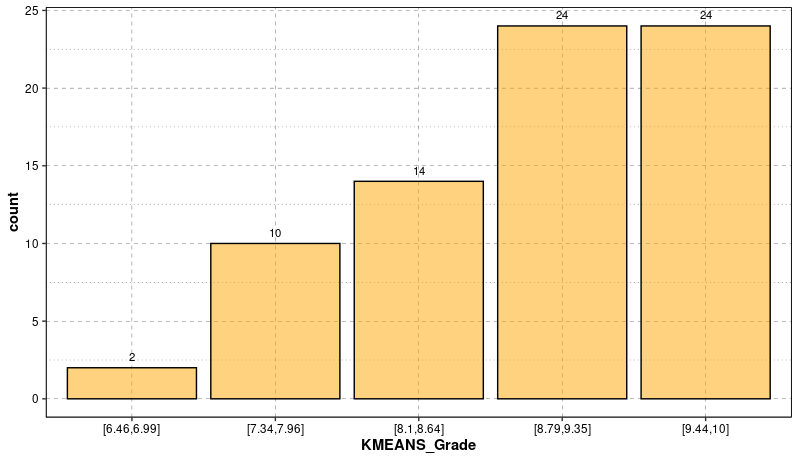
\includegraphics[width=0.47\textwidth]{clustering/KMeans5count.png}}%
\caption{Resultados obtenidos tras aplicar el algoritmo de las $K$-Medias con $K = 5$.}
\label{fig:KMeans5details}
\end{figure}

\section{Por clusters aproximados de rendimiento}

De las medidas de rendimiento estudiadas en el Capítulo \ref{chapter:rendimiento}, nos quedaremos con aquellas que correlan con la variable \emph{Grade} (\emph{np}, \emph{fr}, \emph{ps}, \emph{sq} y \emph{ns}). Así pues, se definirá una nueva métrica como la suma de las medidas de rendimiento \emph{p}, \emph{fr}, \emph{ps}, \emph{sq} y \emph{s}. En la Figura \ref{fig:correlationfm} vemos que ésta no correla con la variable \emph{Grade}.

\begin{figure}[H]
    \centering
    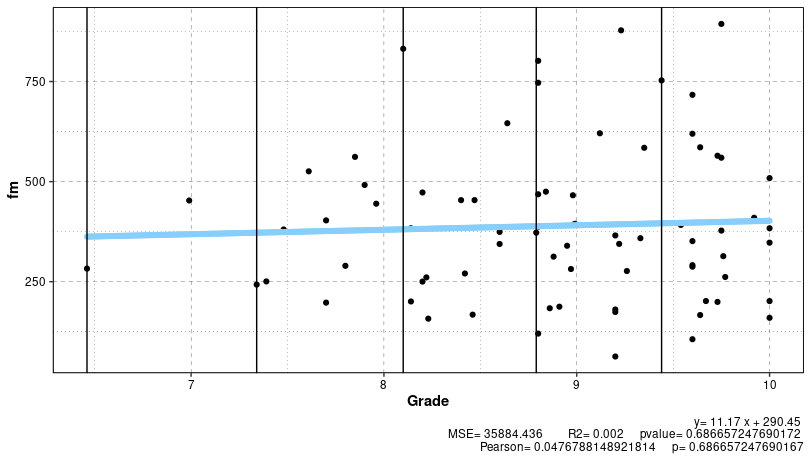
\includegraphics[width=0.8\textwidth]{clustering/fm.png}
    \caption{Regresión lineal para aproximar la relación de dependencia entre la variable \emph{fm} y la variable \emph{Grade}.}
    \label{fig:correlationfm}
\end{figure}

A continuación, se agruparán los datos usando el algoritmo de las K-medias sobre la variable \emph{fm}. Para decidir el número de clusters en el que agruparemos los datos, se usarán métodos gráficos. Como podemos ver en las Figuras \ref{fig:indiceshubertfm} y \ref{fig:indicesdindexfm}, el número óptimo de particiones podría ser $4$ o $7$. Para decidir entre un número de clusters u otro se realizarán los dos agrupamientos y nos quedaremos con el de menor error.

\begin{figure}[H]
    \centering
    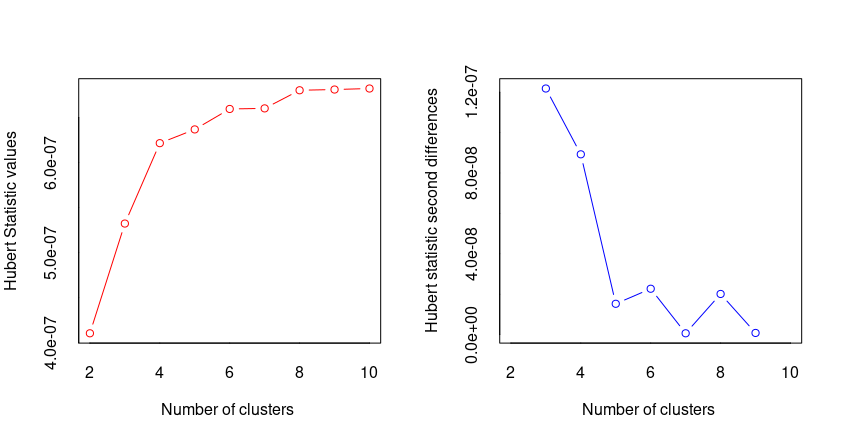
\includegraphics[width=\textwidth]{clustering/Hubertfm.png}
    \caption{Valores estadísticos de Hubert.}
    \label{fig:indiceshubertfm}
\end{figure}

\begin{figure}[H]
    \centering
    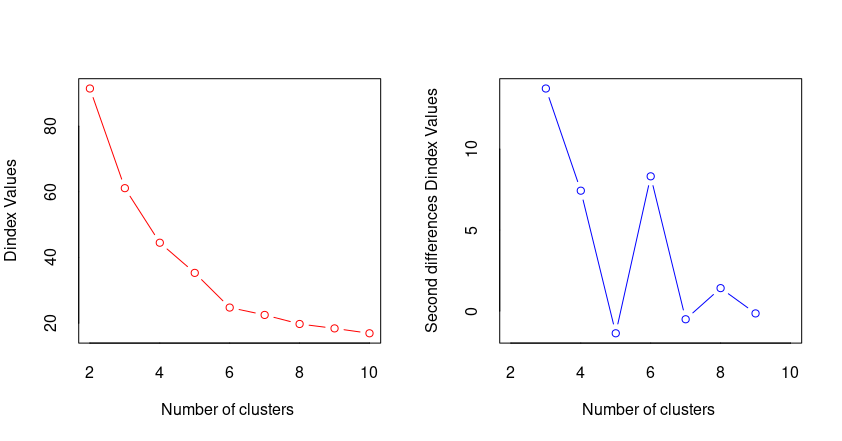
\includegraphics[width=\textwidth]{clustering/Dindexfm.png}
    \caption{Valores de Dindex.}
    \label{fig:indicesdindexfm}
\end{figure}

Aplicando el algoritmo de las K-medias para $K = 4$ (Figura \ref{fig:KMeans4}) y para $K = 7$ (Figura \ref{fig:KMeans7}), vemos que hay una gran diferencia la precisión de uno y otro (para $K = 4$ se tiene $\texttt{accuracy} = 0.921137$ mientras que para $K = 7$ se tendrá $\texttt{accuracy} = 0.9772655$). Además, en la Figura \ref{fig:KMeans4} podemos notar la presencia de outliers mientras que en la Figura \ref{fig:KMeans7} no.

\begin{figure}[H]
    \centering
    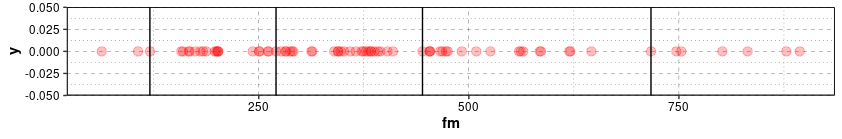
\includegraphics[width=0.6\textwidth]{clustering/outliersfm.png}
    \caption{Particiones obtenidas con $K = 4$. Como podemos ver, se observa la presencia de outliers ($260.804$, $63.173$, $106.379$ y $261.823$).}
    \label{fig:KMeans4}
\end{figure}

\begin{figure}[H]
    \centering
    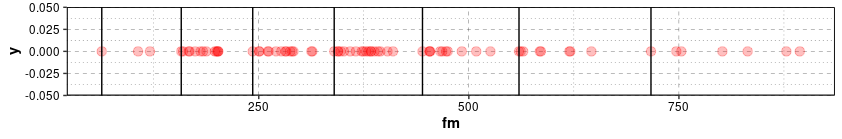
\includegraphics[width=0.6\textwidth]{clustering/KMeans7fm.png}
    \caption{Particiones obtenidas con $K = 7$. No hay ningún outlier.}
    \label{fig:KMeans7}
\end{figure}

La distribución de la variable \emph{Grade} dentro de cada partición puede verse en las Figuras \ref{fig:KMeans4boxplot} y \ref{fig:KMeans7boxplot} mientras que el número de grupo que hay en las particiones puede verse en las Figuras \ref{fig:KMeans4count} y \ref{fig:KMeans7count}.

\begin{figure}[H]
\centering
\subfloat[Boxplot de cada una de las particiones.]{\label{fig:KMeans4boxplot}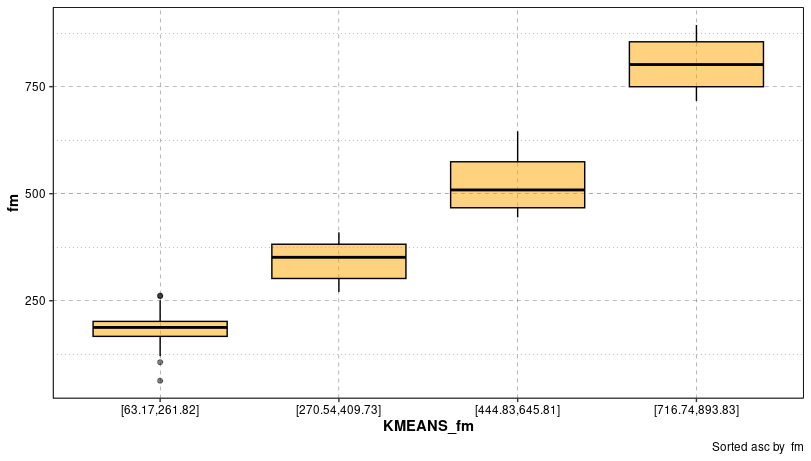
\includegraphics[width=0.47\textwidth]{clustering/KMeansfmboxplot.png}}\qquad
\subfloat[Número de grupos por partición.]{\label{fig:KMeans4count}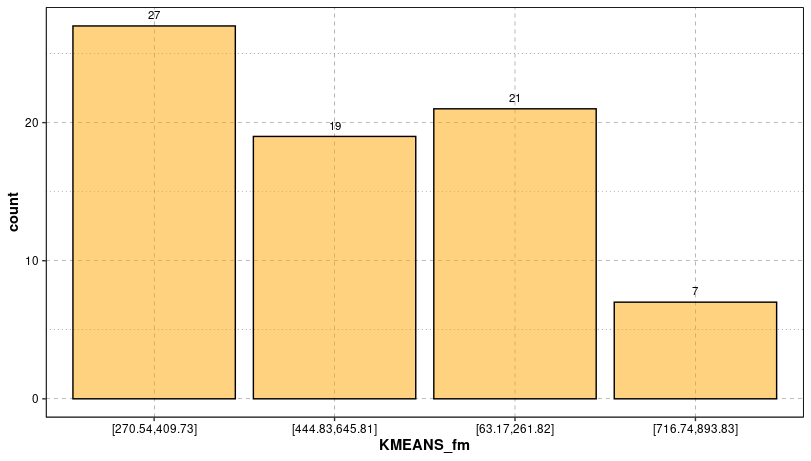
\includegraphics[width=0.47\textwidth]{clustering/KMeansfmcount.png}}%
\caption{Resultados obtenidos tras aplicar el algoritmo de las $K$-Medias con $K = 4$.}
\label{fig:KMeans4details}
\end{figure}

\begin{figure}[H]
\centering
\subfloat[Boxplot de cada una de las particiones.]{\label{fig:KMeans7boxplot}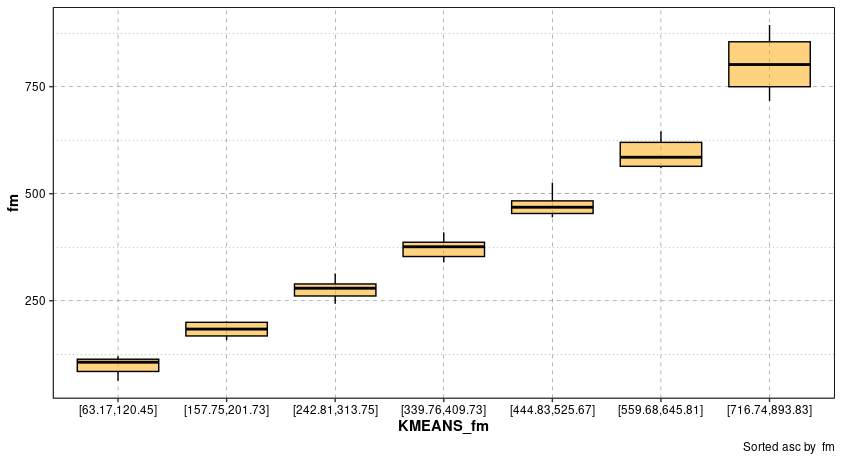
\includegraphics[width=0.47\textwidth]{clustering/KMeans7boxplot.png}}\qquad
\subfloat[Número de grupos por partición.]{\label{fig:KMeans7count}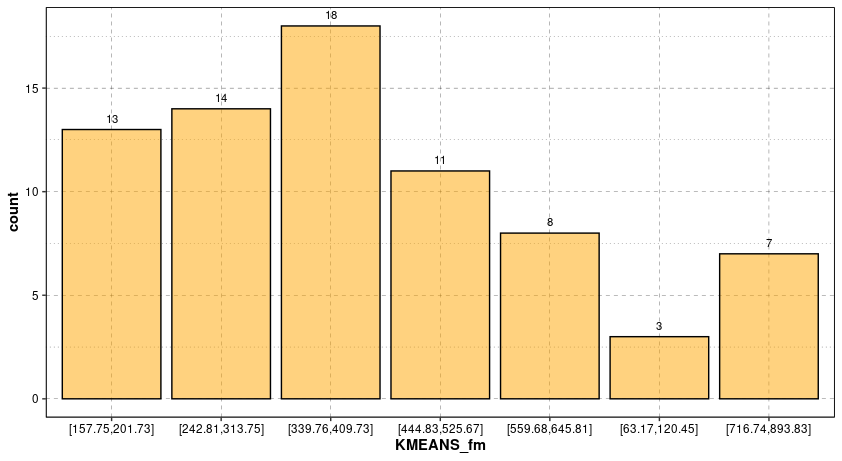
\includegraphics[width=0.47\textwidth]{clustering/KMeans7count.png}}%
\caption{Resultados obtenidos tras aplicar el algoritmo de las $K$-Medias con $K = 7$.}
\label{fig:KMeans7details}
\end{figure}

\section{Clustering mediante las propiedas espectrales de los grafos}
\subsection{Clustering mediante el coeficiente LOGLAP09}

Ahora, se ha decidido se asociar los datos usando el algoritmo de las K-medias sobre la variable \emph{LOGLAP09}. Para decidir el número de clusters en el que agruparemos los datos, se usarán métodos gráficos. Como podemos ver en las Figuras \ref{fig:indiceshubertLAP} y \ref{fig:indicesdindexLAP}, se ha decidido agrupar los datos en $5$ clusters (Figura \ref{fig:KMeansLAP}, $\texttt{accuracy} = 0.9673813$).

\begin{figure}[H]
    \centering
    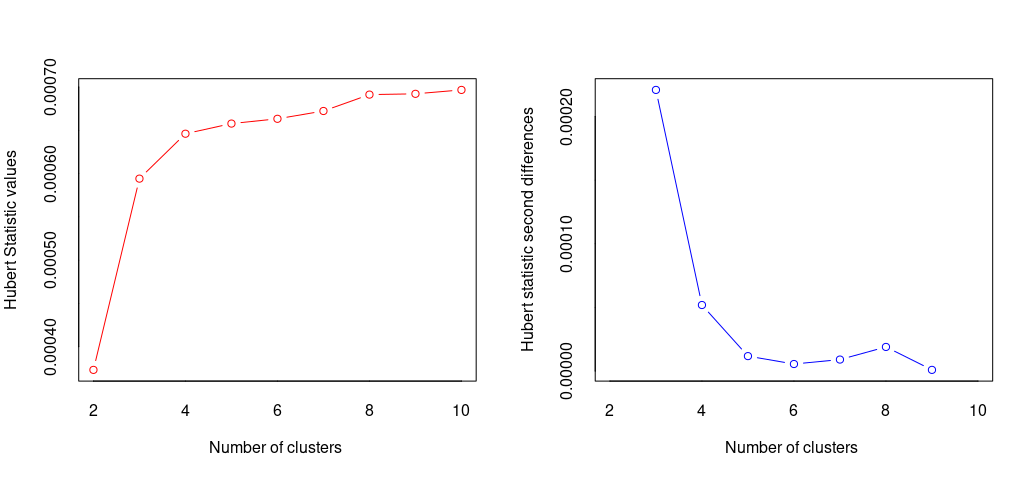
\includegraphics[width=\textwidth]{clustering/HubertLAP.png}
    \caption{Valores estadísticos de Hubert.}
    \label{fig:indiceshubertLAP}
\end{figure}

\begin{figure}[H]
    \centering
    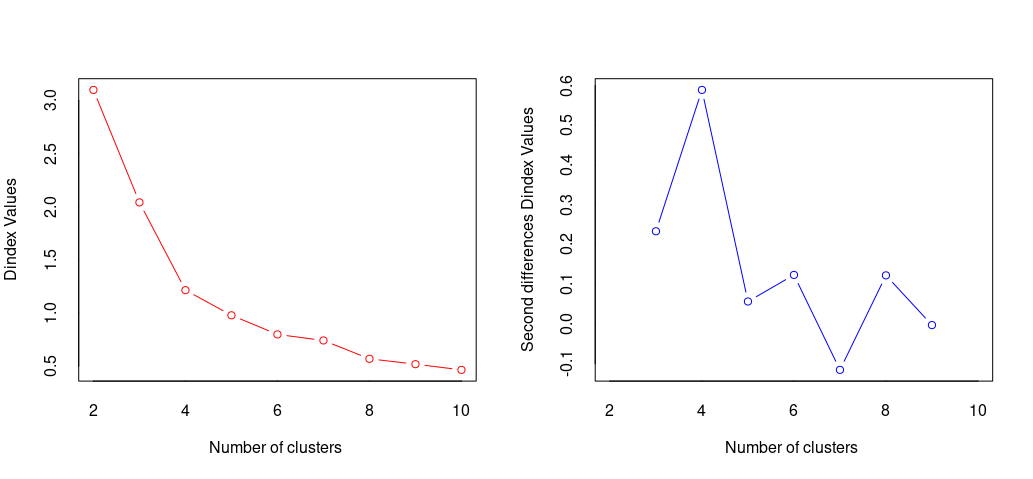
\includegraphics[width=\textwidth]{clustering/DindexLAP.png}
    \caption{Valores de Dindex.}
    \label{fig:indicesdindexLAP}
\end{figure}

\begin{figure}[H]
    \centering
    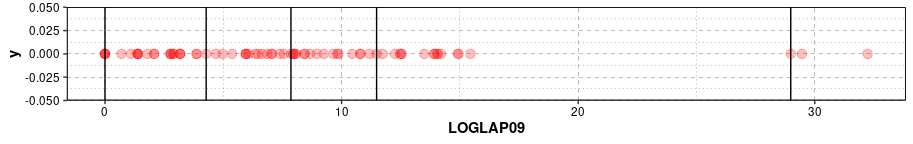
\includegraphics[width=0.6\textwidth]{clustering/partitionsLOGLAP09.png}
    \caption{Particiones obtenidas con $K = 5$. No hay ningún outlier.}
    \label{fig:KMeansLAP}
\end{figure}

La distribución de la variable \emph{Grade} dentro de cada partición puede verse en la Figura \ref{fig:KMeansLAPboxplot} mientras que el número de grupos que hay en las particiones puede verse en la Figura \ref{fig:KMeansLAPcount}.

\begin{figure}[H]
\centering
\subfloat[Boxplot de cada una de las particiones.]{\label{fig:KMeansLAPboxplot}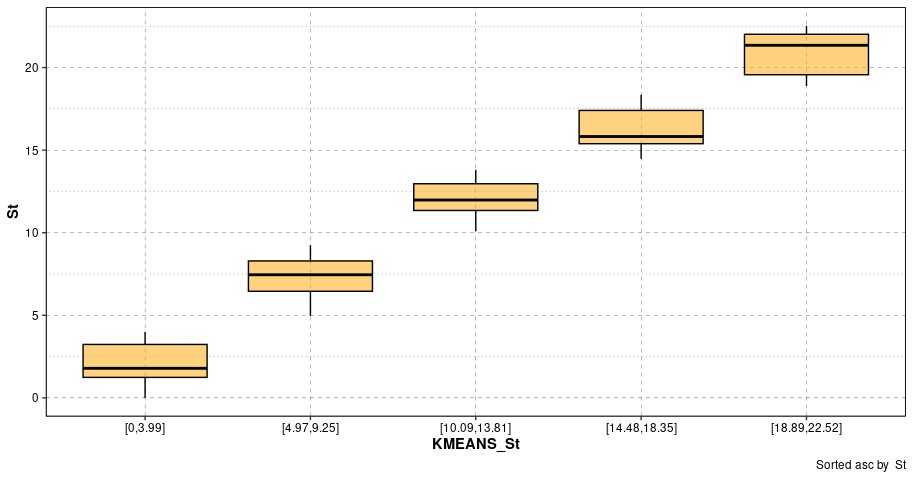
\includegraphics[width=0.47\textwidth]{clustering/KMeansLAPboxplot.png}}\qquad
\subfloat[Número de grupos por partición.]{\label{fig:KMeansLAPcount}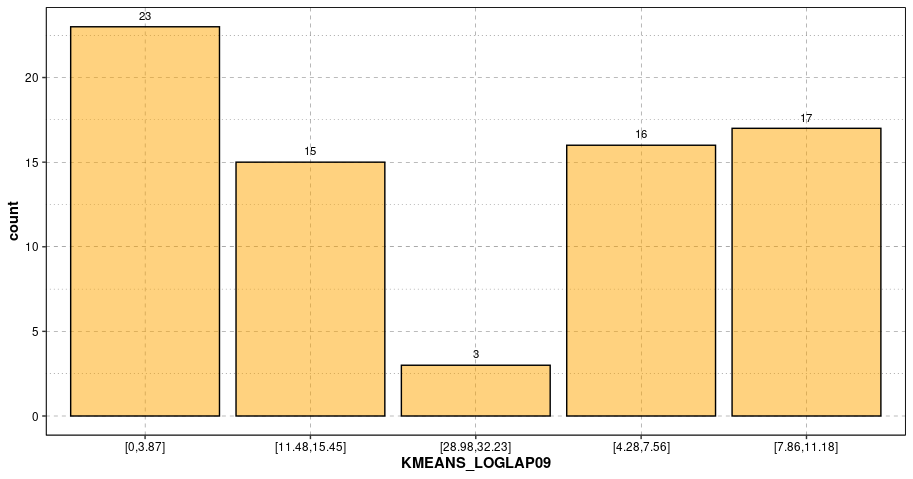
\includegraphics[width=0.47\textwidth]{clustering/KMeansLAPcount.png}}%
\caption{Resultados obtenidos tras aplicar el algoritmo de las $K$-Medias con $K = 5$.}
\label{fig:KMeansLAPdetails}
\end{figure}

\subsection{Clustering mediante el coeficiente DAG}